%%%%%%%%%%%%%%%%%%%%%%%%%%%%%%%%%%%%%%%%%%%%%%%%%%%%%%%%%%%%%%%%%%%%%%%%%%%%%%%%%%%%%%%%%%%%%%
%% Chapter 1

%% Set chapters counter to zero.
\setcounter{chapter}{0}

\chapter{\MakeUppercase{Literature review / Literatūros apžvalga}} %Make it upper case to appear in TOC correctly
\label{cha:review}

%%%%%%%%%%%%%%%%%%%%%%%%%%%%%%%%%%%%%%%%%%%%%%%%%%%%%%%%%%%%%%%%%%%%%%%%%%%%%%%%%%%%%%%%%%%%%%
%%  Text / Tekstas

A literature review surveys prior research published in books, scholarly articles, and any other sources relevant to a particular issue, area of research, or theory, and by so doing, provides a description, summary, and critical evaluation of these works in relation to the research problem being investigated. Literature reviews are designed to provide an overview of sources you have used in researching a particular topic and to demonstrate to your readers how your research fits within existing scholarship about the topic.  (Fink, Arlene. Conducting Research Literature Reviews: From the Internet to Paper. Fourth edition. Thousand Oaks, CA: SAGE, 2014.)\footnote{https://libguides.usc.edu/writingguide/literaturereview}. 

You should rename the title of this chapter to fit your dissertation domain. 

It must describe the research conducted on the topic of the dissertation in Lithuania and abroad and show the contribution of the author of the dissertation to the issue under consideration.
Although there are no formal requirements for the review, it is recommended that it be no longer than 50\% of the entire text of the dissertation (excluding the introduction). The recommended volume of the literature review is 33\% of the entire dissertation text.

\textbf{In Lithuanian}. Literatūros apžvalga, tai apžvalga ir tyrimas: knygų, mokslinių straipsnių ir kitų susijusių su pasirinkta tyrimo problema šalinių, tyrimo srities, teorijos. 
Literatūros apžvalga leidžia apibrėžti, apibendrinti ir kritiškai įvertinti darbus susijusius su norima tirti tyrimo problema.
Literatūros apžvalga leidžia pademonstruoti skaitytojams kad jūsų tyrimas priklauso platesniam tyrimų ratui, sričiai. (Fink, Arlene. Conducting Research Literature Reviews: From the Internet to Paper. Fourth edition. Thousand Oaks, CA: SAGE, 2014.) 


Šio skyriaus pavadinimas parenkamas taip, kad atitiktų apžvalgą disertacijos srityje.

Tyrimų apžvalga.\index{Tyrimų apžvalga} Joje turi būti aprašyti disertacijos tema \textbf{Lietuvoje ir užsienyje atlikti tyrimai} ir parodyta, koks yra disertacijos autoriaus indėlis į nagrinėjamą problematiką.

Nors formalių reikalavimų apžvalgai nėra, tačiau rekomenduojama kad ji būtų ne ilgesnė negu 50\% viso disertacijos teksto (atmetus įvadą). Rekomenduojama literatūros apžvalgos apimtis 33\% viso disertacijos teksto.


\section{How to use \LaTeX{} / Kaip galima panaudoti \LaTeX{}?}
\label{sec:intro_latex}

The thesis is composed of each chapters that are themselves composed of sections, sub-sections, etc.
To create such a heading structure, you can use the commands \verb|\chapter{}|, \verb|\section{}|, \verb|\subsection{}|, \verb|\subsubsection{}|, and \verb|\paragraph{}|. 
Note that, while \verb|\section{}| should be inside a \verb|\chapter{}|, a \verb|\subsection{}| inside a \verb|\section{}|, etc., a \verb|\paragraph{}| is not numbered and can thus be added inside any of those.

If you wish to cross-reference a heading elsewhere in the text, you will need to do two things. 
First you must give that heading a \emph{label} using the command \verb|\label{}|, e.g. \verb|\label{sec:TextStructure}|. This label should be put right after the heading declaration: either on the same line or the next one.
Then, you can cross-reference the heading in the text using commands like \verb|\cref{}|.
More information about cross-referencing can be found in \Cref{sec:crossreferencing}.


 \cite{demoABook, demoArticle}.

This template supports four levels of section: \verb|\chapter{}|,
\verb|\section{}|, \verb|\subsection{}| and \verb|subsubsection{}|.


\section{A Section} \label{sec:section}

\subsection{A Sub-section}  \label{subs:subsection}

\subsubsection{A Sub-sub-section}  \label{subs:subsubsection}


\section{Usage of tables / Lentelių panaudojimas}

\begin{table}[ht!]
  \centering
  \caption{Kinetic constants and thermodynamic parameters for the GOx catalyzed reaction with $\beta$-D-glucose and oxygen at pH 5.5.}
  \label{tab:const}  
  \vspace{2mm} 
  \def\arraystretch{1.1}
  \begin{tabular}{ | m{8em} | c | c | c | c | c |}
    \hline
    Sugar substrate or thermodynamic parameter & \begin{tabular}{@{}c@{}} $k_{1}$,\\ \si{M^{-1}s^{-1}}\end{tabular} & $k_{2}$, \si{s^{-1}} & \begin{tabular}{@{}c@{}}  $k_{3}$,\\ \si{M^{-1}s^{-1}} \end{tabular} & $k_{4}$, \si{s^{-1}} & ref. \\ \hline
    $\beta$-D-glucose-1-\ce{^1H} at \SI{25}{\degreeCelsius} & ${\sim}200$ & ${\sim}\num{6000}$ & $\num{1.8d6}$ & $\num{1440}$ & \\ \hline
    $\beta$-D-glucose-1-\ce{^1H} at \SI{25}{\degreeCelsius} & $\num{13158}$ & & $\num{1.8d6}$ &  $\num{1440}$ & \\ \hline
    $\beta$-D-glucose-1-\ce{^1H} at \SI{27}{\degreeCelsius} & $\num{10000}$ & & $\num{2.1d6}$ & $\num{1150}$ & \\ 
\hline
    % \midrule
    Used in the model & $\num{3000}$ & $\num{6000}$ & $\num{1.5d6}$ & $\num{1500}$ & \\ [1ex]
    \hline
  \end{tabular}
\end{table}


\section{Figures}  \label{sec:figures}

\begin{figure}[ht!]
\centering
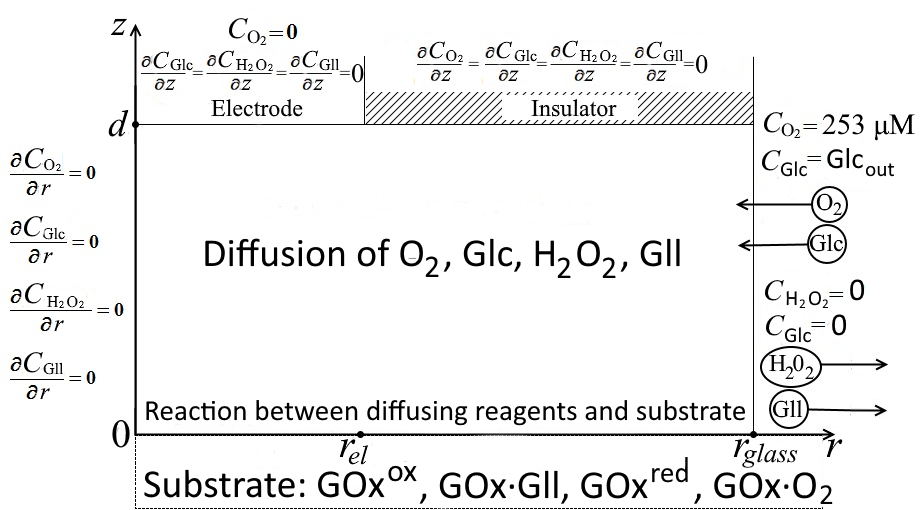
\includegraphics[width=1\linewidth]{chapter_1/Model_domain.png}
\caption{Scheme of simulation domain. All 8 reagents, boundary conditions for $C_{\text{diff}}$ and the direction of outside flux are displayed.}
\label{fig:Domain}
\end{figure}

Measurements of SECM acting in the redox-competition mode are changed into the scheme (\ref{fig:Domain}) due to the radial symmetry around the central axis of the electrode. Radial symmetry is a standard assumption in SECM modelling, though the case of off-centered UME was also investigated.


\section{Equations}  \label{sec:equations}
According to the second Fick’s law , diffusion processes are expressed by the system of partial differential equations (PDE):

\begin{equation}
  \begin{aligned}\label{eq:reakc_eq1}
  \frac{\partial C_{O_2}}{\partial t} &= D_{O_2}\,\Delta C_{O_2},\\
  \frac{\partial C_{Glc}}{\partial t} &= D_{Glc}\,\Delta C_{Glc},\\
  \frac{\partial C_{H_2 O_2}}{\partial t} &= D_{H_2 O_2} \,\Delta C_{H_2 O_2},\\
  \frac{\partial C_{Gll}}{\partial t} &= D_{Gll}\,\Delta C_{Gll},  \quad for\; 0<t\leq T,\; 0<z<d,\; 0<r<r_{glass},
  \end{aligned}
\end{equation}

where:
\begin{itemize}
  \item[] $C_{O_2}$, $C_{Glc}$, $C_{H_2 O_2}$ and $ C_{Gll}$ are concentrations of diffusing reagents and expressed as functions of time $t$ and spatial coordinates $z$ and $r$. Notation $C_{\text{diff}} = C_{\text{diff}} \left( t, z, r \right) = \left( C_{O_2}, C_{Glc}, \allowbreak C_{H_2 O_2}, \allowbreak C_{Gll} \right)$ was used when 4 diffusing re\-agents were considered together.
  \item[] $D_{O_2}$, $D_{Glc}$, $D_{H_2 O_2}$ and $D_{Gll}$ are diffusion coefficients of \ce{O2}, Glc, \ce{H2O2} and Gll.
  \item[] $d$ is the distance between the enzyme-modified surface and the electrode, which is varying from \SIrange{1}{120}{\um} as shown in Fig. \ref{fig:Domain}.
  \item[] $r_{glass} = \SI{80}{\um}$ is the radius of insulated area, $r_{el} = \SI{5}{\um}$ is the radius of electrode.
  \item[] $T$ is the duration of a computational experiment measured in seconds (the evaluation of this parameter is further explained in the next section).
  \item[] The Laplace operator $\Delta$ for concentration function $C$ in cylindrical coordinates with radial symmetry is
  \begin{equation*}
  \Delta C = \frac{1}{r}\frac{\partial }{\partial r} \left( r\frac{\partial C }{\partial r} \right) + \frac{\partial^{2} C}{\partial z^{2}}.
  \end{equation*}
\end{itemize}


\subsection{Lists}
\label{subsec:lists}

\begin{enumerate}
  \item Numbered lists should be presented using the environment \verb|enumerate| like in this example. 
  This environment applies the numbering and defines the format and spacing automatically. 
  % \item Add the option \verb|[noitemsep]| to the environment to have no additional space between numbered list items (like is done here).
\end{enumerate}

\begin{itemize}
  \item Bulleted lists should be presented using the environment \verb|itemize| like in this example. 
  This environment applies the numbering and defines the format and spacing automatically. 
  % \item Add the option \verb|[noitemsep]| to the environment to have no additional space between bulleted list items  (this is not done here).
\end{itemize}
